% !TEX encoding = UTF-8
% !TEX TS-program = pdflatex
% !TEX root = ../tesi.tex

%**************************************************************
\chapter{L'azienda}
\label{cap:azienda}

\section{Descrizione}

WorkWave, una divisione di IFS, è una società americana fondata nel 1984 con anche sede in Italia che fornisce soluzioni di Field Service Management e che connette ogni aspetto di un business attraverso le sue piattaforme unificate e di facile uso. L'insieme delle soluzioni della compagnia permettono ai professionisti di servizi ultimo-miglio di facilmente assegnare ed automatizzare attività di vendita e marketing, migliorando l'efficienza ed incrementando la visibilità delle operazioni sul campo attraverso le soluzioni mobile. \\

Le piattaforme di WorkWave forniscono ad oltre 8 mila clienti un livello senza precedenti di analisi del business, permettendolo loro di aumentare l'efficienza, il guadagno e garantendo un'eccezionale customer experience.

\begin{figure}[H] 
  \centering 
  
\includegraphics[]{workwave-logo} 
  \caption{Logo dell'azienda WorkWave}
\end{figure}

\section{Servizi offerti}

WorkWave aiuta aziende nel campo Field Service Management ed industrie di trasporti e logistica mitigare gli aspetti dolorosi che incontrano ogni giorno, consentendo loro di salvare tempo, spese e migliorando il servizio agli utenti. Per Field Service Management si intendono risorse impiegate per intradare verso i domicili dei clienti, quali localizzazione dei veicoli, gestione delle attività degli operatori, pianificazione ed impiego delle attività, garanzia della sicurezza dei conducenti ed integrazione di tali servizi con depositi, fatturazione ed altri servizi back-office. \\

WorkWave fornisce sia soluzioni per l'installazione e manutenzione hardware che servizi software per l'aiuto della gestione di tali attività. \\

La suite dei servizi software cloud, mobile e marketing permette a compagnie di ogni dimensione di facilmente stimare attività, pianificare ed dirigere operatori mobili con facilità. Di seguito si elencano i principali correlati all'attività di stage:

\begin{itemize}
  \item \textit{WorkWave Service}: è un servizio software che consente ti velocemente schedulare rotte efficienti, visionare la produttività in tempo reale degli operatori, visualizzare stime e gestire pagamenti;
  \item \textbf{WorkWave Route Manager}: è un set di servizi per la gestione dei veicoli al fine di migliorare l'efficienza e la scalabilità attraverso pianificazione dinamica e miglioramenti intelligenti delle rotte. L'algoritmo proprietario del Route Manager garantisce che le migliori rotte per gli operatori siano usate per salvare tempo, costi e migliorare la soddisfazione dei clienti;
  \item \textbf{WorkWave GPS}: fornisce un'intuitiva panoramica dei propri veicoli e delle propie risorse con un potente servizio GPS che cattura le azioni dell'operatore e le posizioni in tempo reale dei veicoli. Permette inoltre di migliorare la sicurezza dei guidatori, segnalare comportamenti errati e riportare incidenti per velocità, frenata improvvisa, curve o altro.
\end{itemize}

\section{Route Manager}

\begin{figure}[h] 
  \centering 
  
\includegraphics[width=0.5\columnwidth]{workwave-route-manager-logo} 
  \caption{Logo WorkWave Route Manager}
\end{figure}

WorkWave Italy è la sede italiana di WorkWave dove sono concentrati gli sviluppi dell'algoritmo di routing e del Route Manager nella nuova versione denominata Unified UI, contesto di sviluppo delle attività dello stage descritte in questo documento.
WorkWave Route Manager automatizza la pianificazione delle rotte per migliorarne l'efficienza e la comunicazione tra l'amministrazione e i guidatori dei veicoli, completamente customizzabile tramite le sue API. \\

\begin{figure}[H] 
  \centering 
  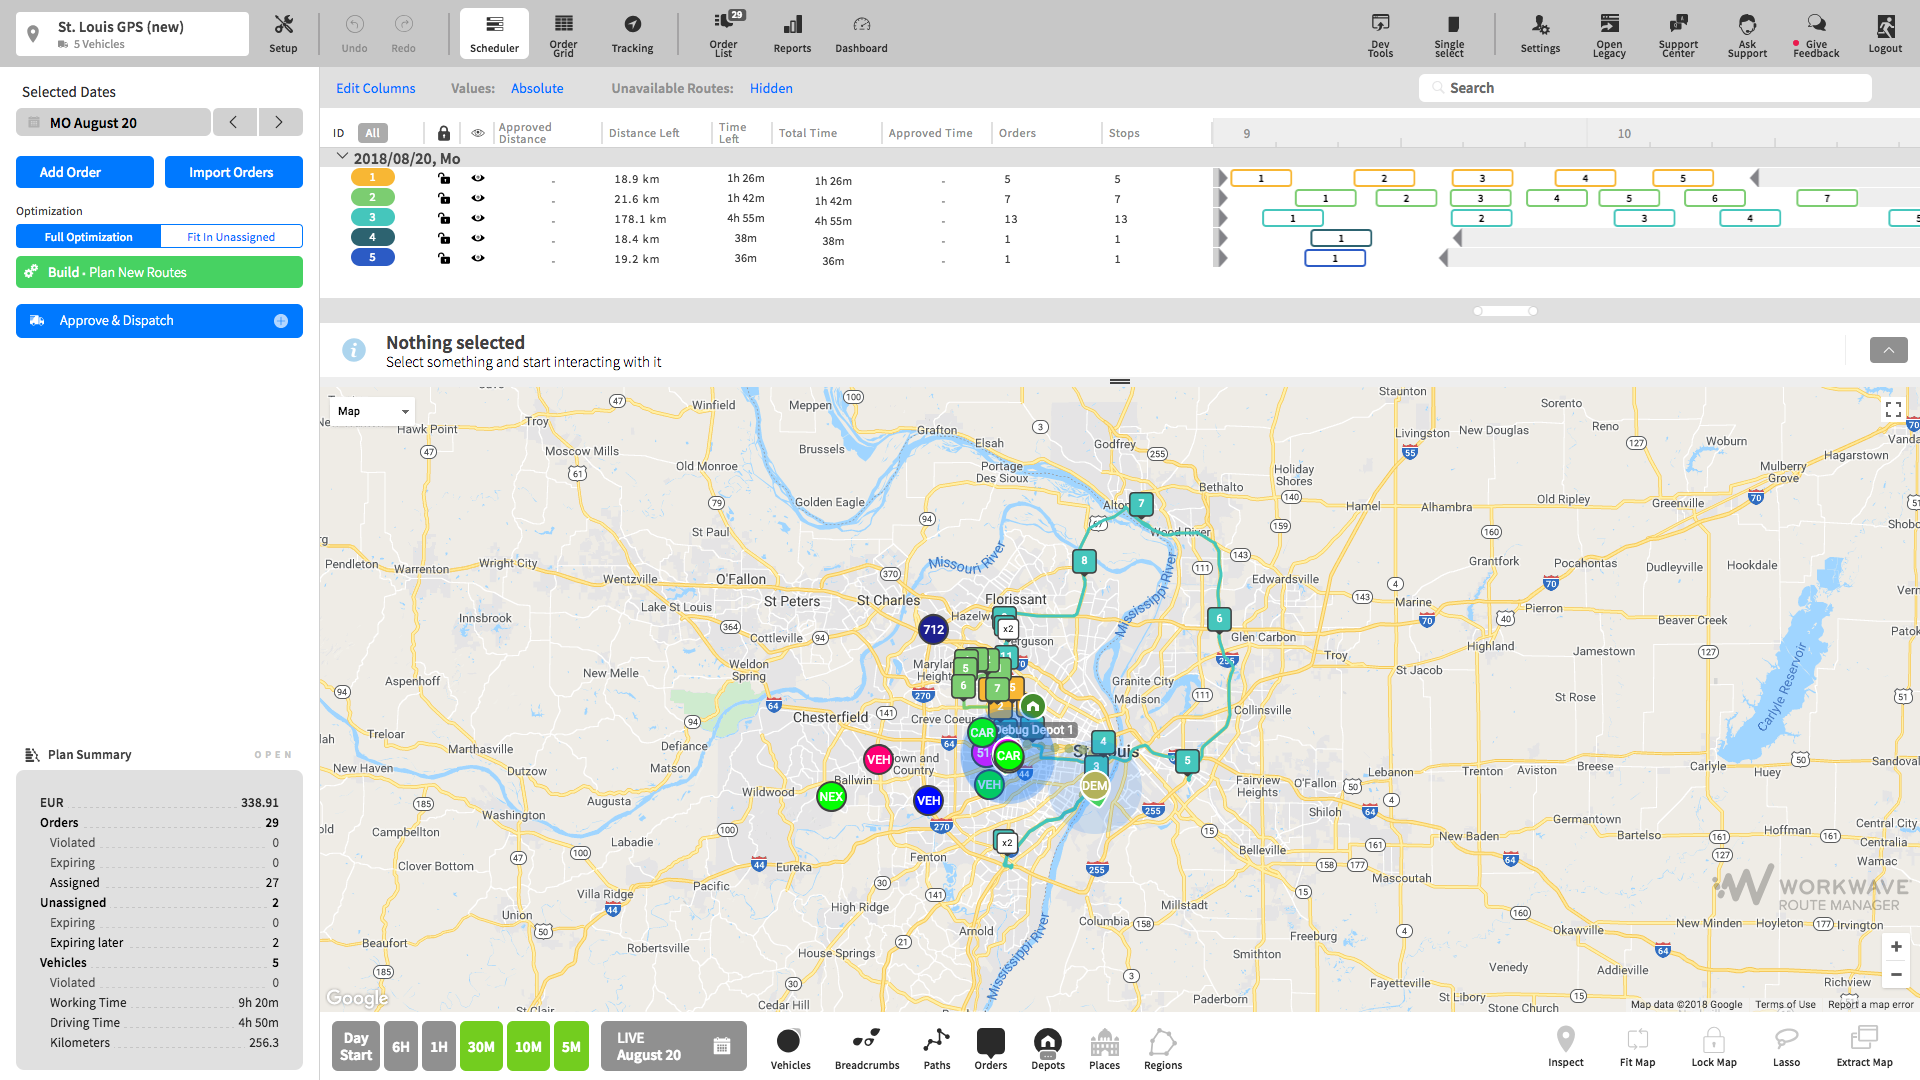
\includegraphics[width=1\columnwidth]{route-manager} 
  \caption{WorkWave Route Manager - Unified UI}
\end{figure}

In particolare, per quanto riguarda Routing \& Scheduling, rende possibile navigare attraverso le richieste dei clienti per gli orari di ricezione, schedulare le attività dei guidatori giornalmente ed eseguire report sulle performance. Attraverso le impostazioni, il software fornisce rotte ottimali in base ai propri vincoli stradali. \\

È inoltre possibile fare aggiustamenti manuali alle rotte via drag\&drop, approvare i piani e mandarli in esecuzione agli operatori sui veicoli. Oltre a ciò consente di visualizzare istantaneamente gli effetti sul numero di ordini possibili per i veicoli disponibili, il tempo stimato di completamento delle attività e comparare il costo per miglio.

\begin{figure}[H] 
  \centering 
  
\includegraphics[width=1\columnwidth]{rm-scheduler} 
  \caption{WorkWave Route Manager - Scheduler degli ordini}
\end{figure}
